\documentclass[aspectratio=43]{beamer}

\usepackage{amsmath, amsthm, amssymb}
\usepackage{empheq}
\usepackage{xcolor}
\newcommand{\R}{\mathbb{R}}
\usepackage{natbib}
\bibliographystyle{plain}


\title{Dimension reduction for single-cell and spatial RNA-seq using generalized bilinear models}
\author{\texorpdfstring{Phillip Nicol \\ Department of Biostatistics, Harvard University}{}}
\institute{NESS 2024 (Storrs, CT)}
\date{May 24, 2024}

\begin{document}

\titlepage

\begin{frame}{Introduction}

\begin{itemize}
\item Single-cell RNA-seq is a revolutionary technology that allows gene expression to be quantified at the level of individual cells. 

\item Data comes in the form of $I \times J$ count matrix $Y$. 

\item For large datasets $I \approx 10^4$ and $J \approx 10^7$. 

\item Dimension reduction is a critical first step before downstream analysis (clustering, visualization, etc.) 

\centering
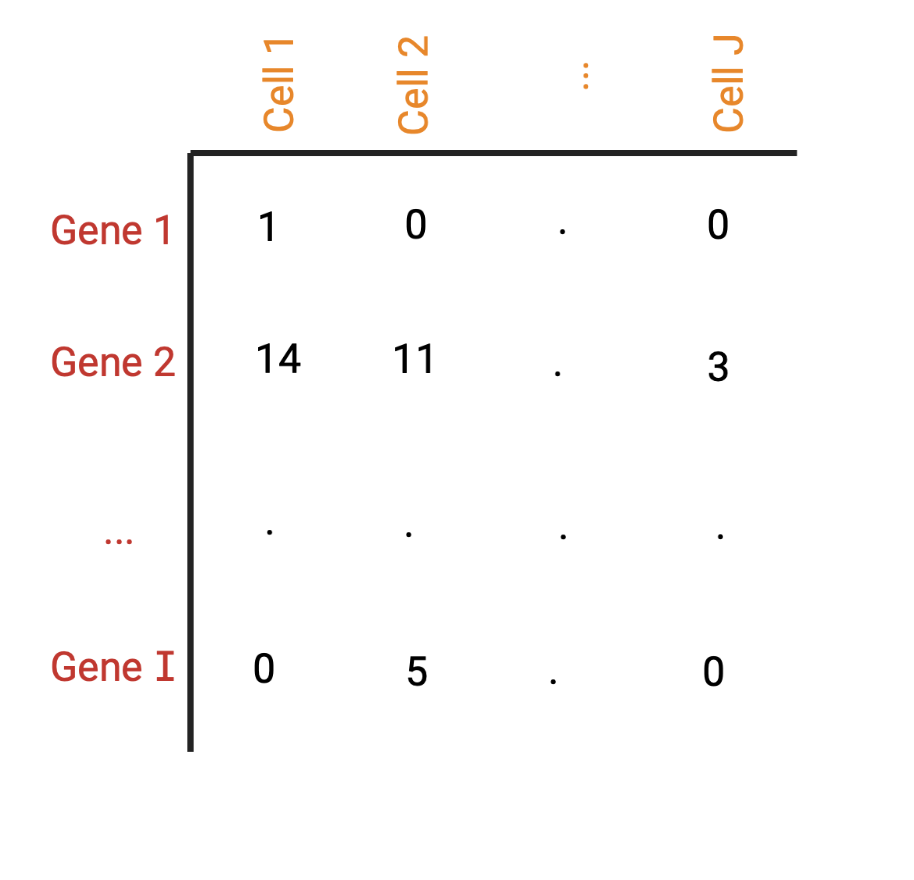
\includegraphics[scale=0.6]{Fig/counts.png}

\end{itemize}
\end{frame}

\begin{frame}{PCA cannot be directly applied due to heterogeneous variances}
\centering 
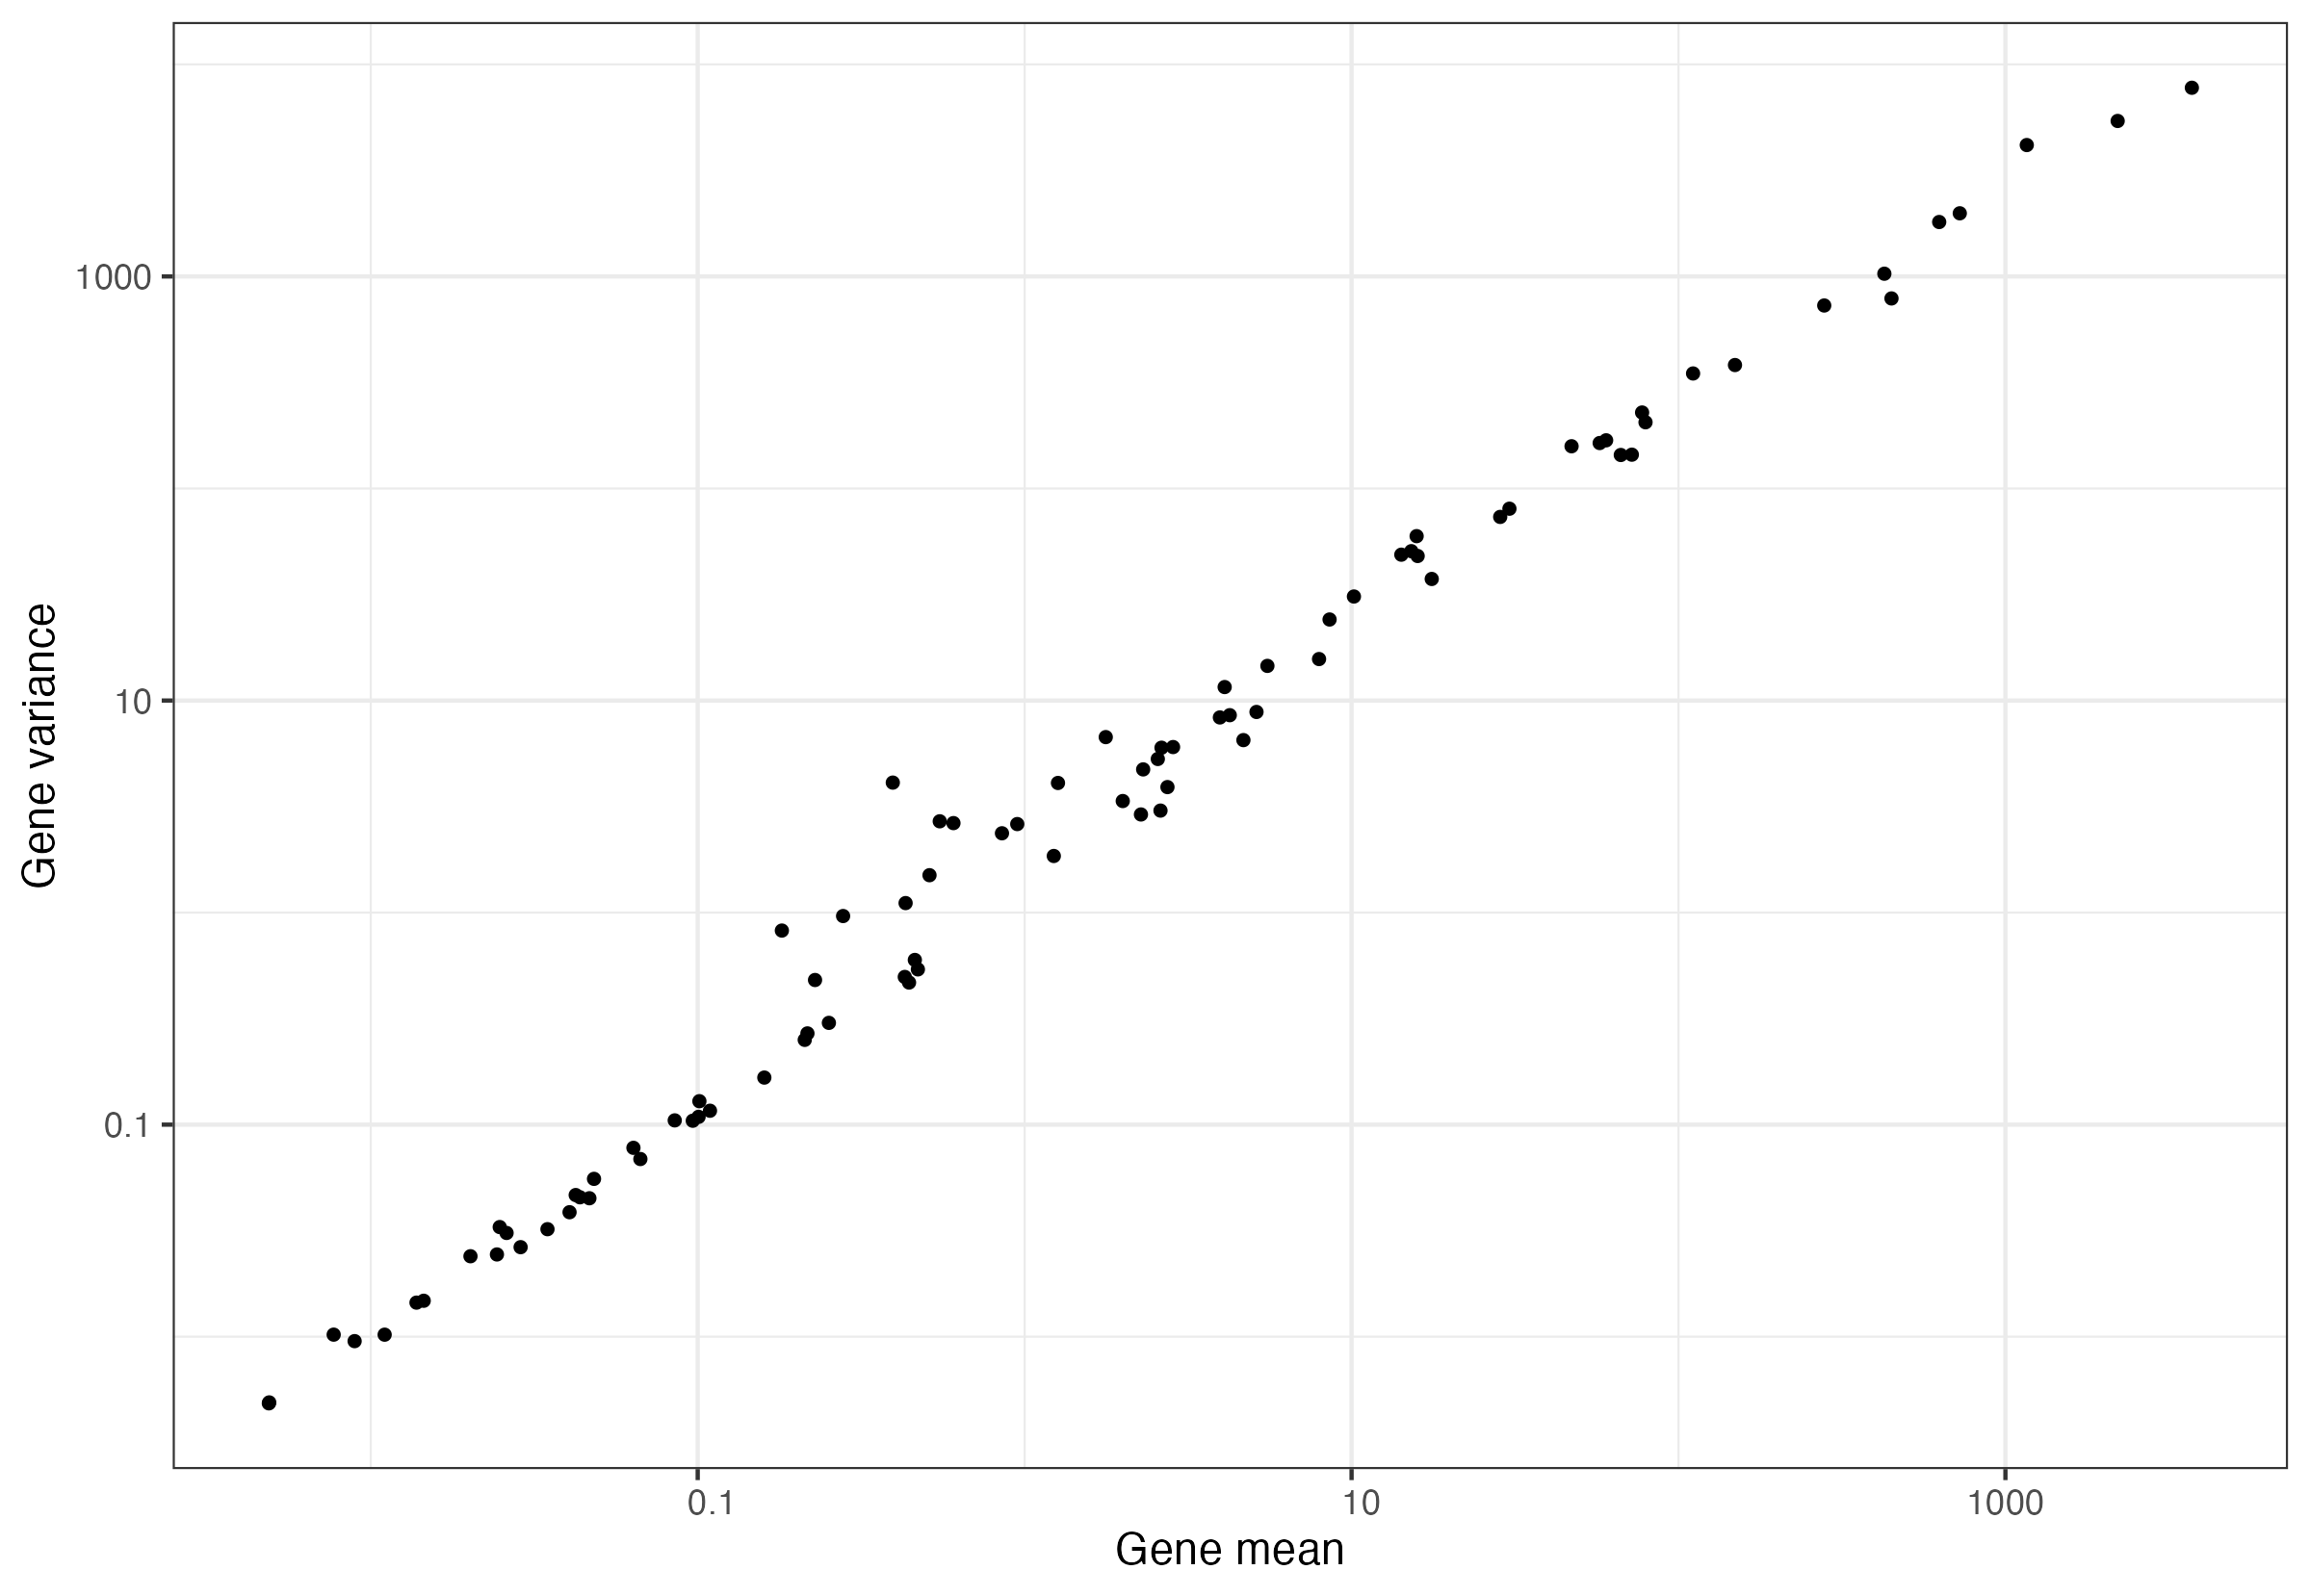
\includegraphics[scale=0.4]{Fig/mean_variance_relationship.png}
\end{frame}

\begin{frame}{Standard approach is to transform the counts prior to PCA}

The counts are commonly pre-processed by computing the \textit{Pearson residual}:

\begin{equation}
Z_{ij} := \frac{Y_{ij} - \hat{\mu}_{i}}{\sqrt{ \hat{\mu}_{i} - \hat{\alpha}_i \hat{\mu}_{i}^2}}
\end{equation}

\begin{itemize}
\item scTransform (SCT) \cite{hafemeister2019normalization}: Estimate $\hat{\mu}$ and $\hat{\alpha}$ with a NB GLM.
\item APR \cite{lause2021analytic}: Fix $\hat{\alpha} = 0.01$ and use a closed-form approximation to $\hat{\mu}$. 
\end{itemize}
\end{frame}

\begin{frame}{PCA on Pearson residuals can fail to capture rare cell types}
If $\hat{\mu}_i$ is large then $Z_{ij} \approx Z_{ij'}$ even for very different counts.

\vspace{2em}

\centering
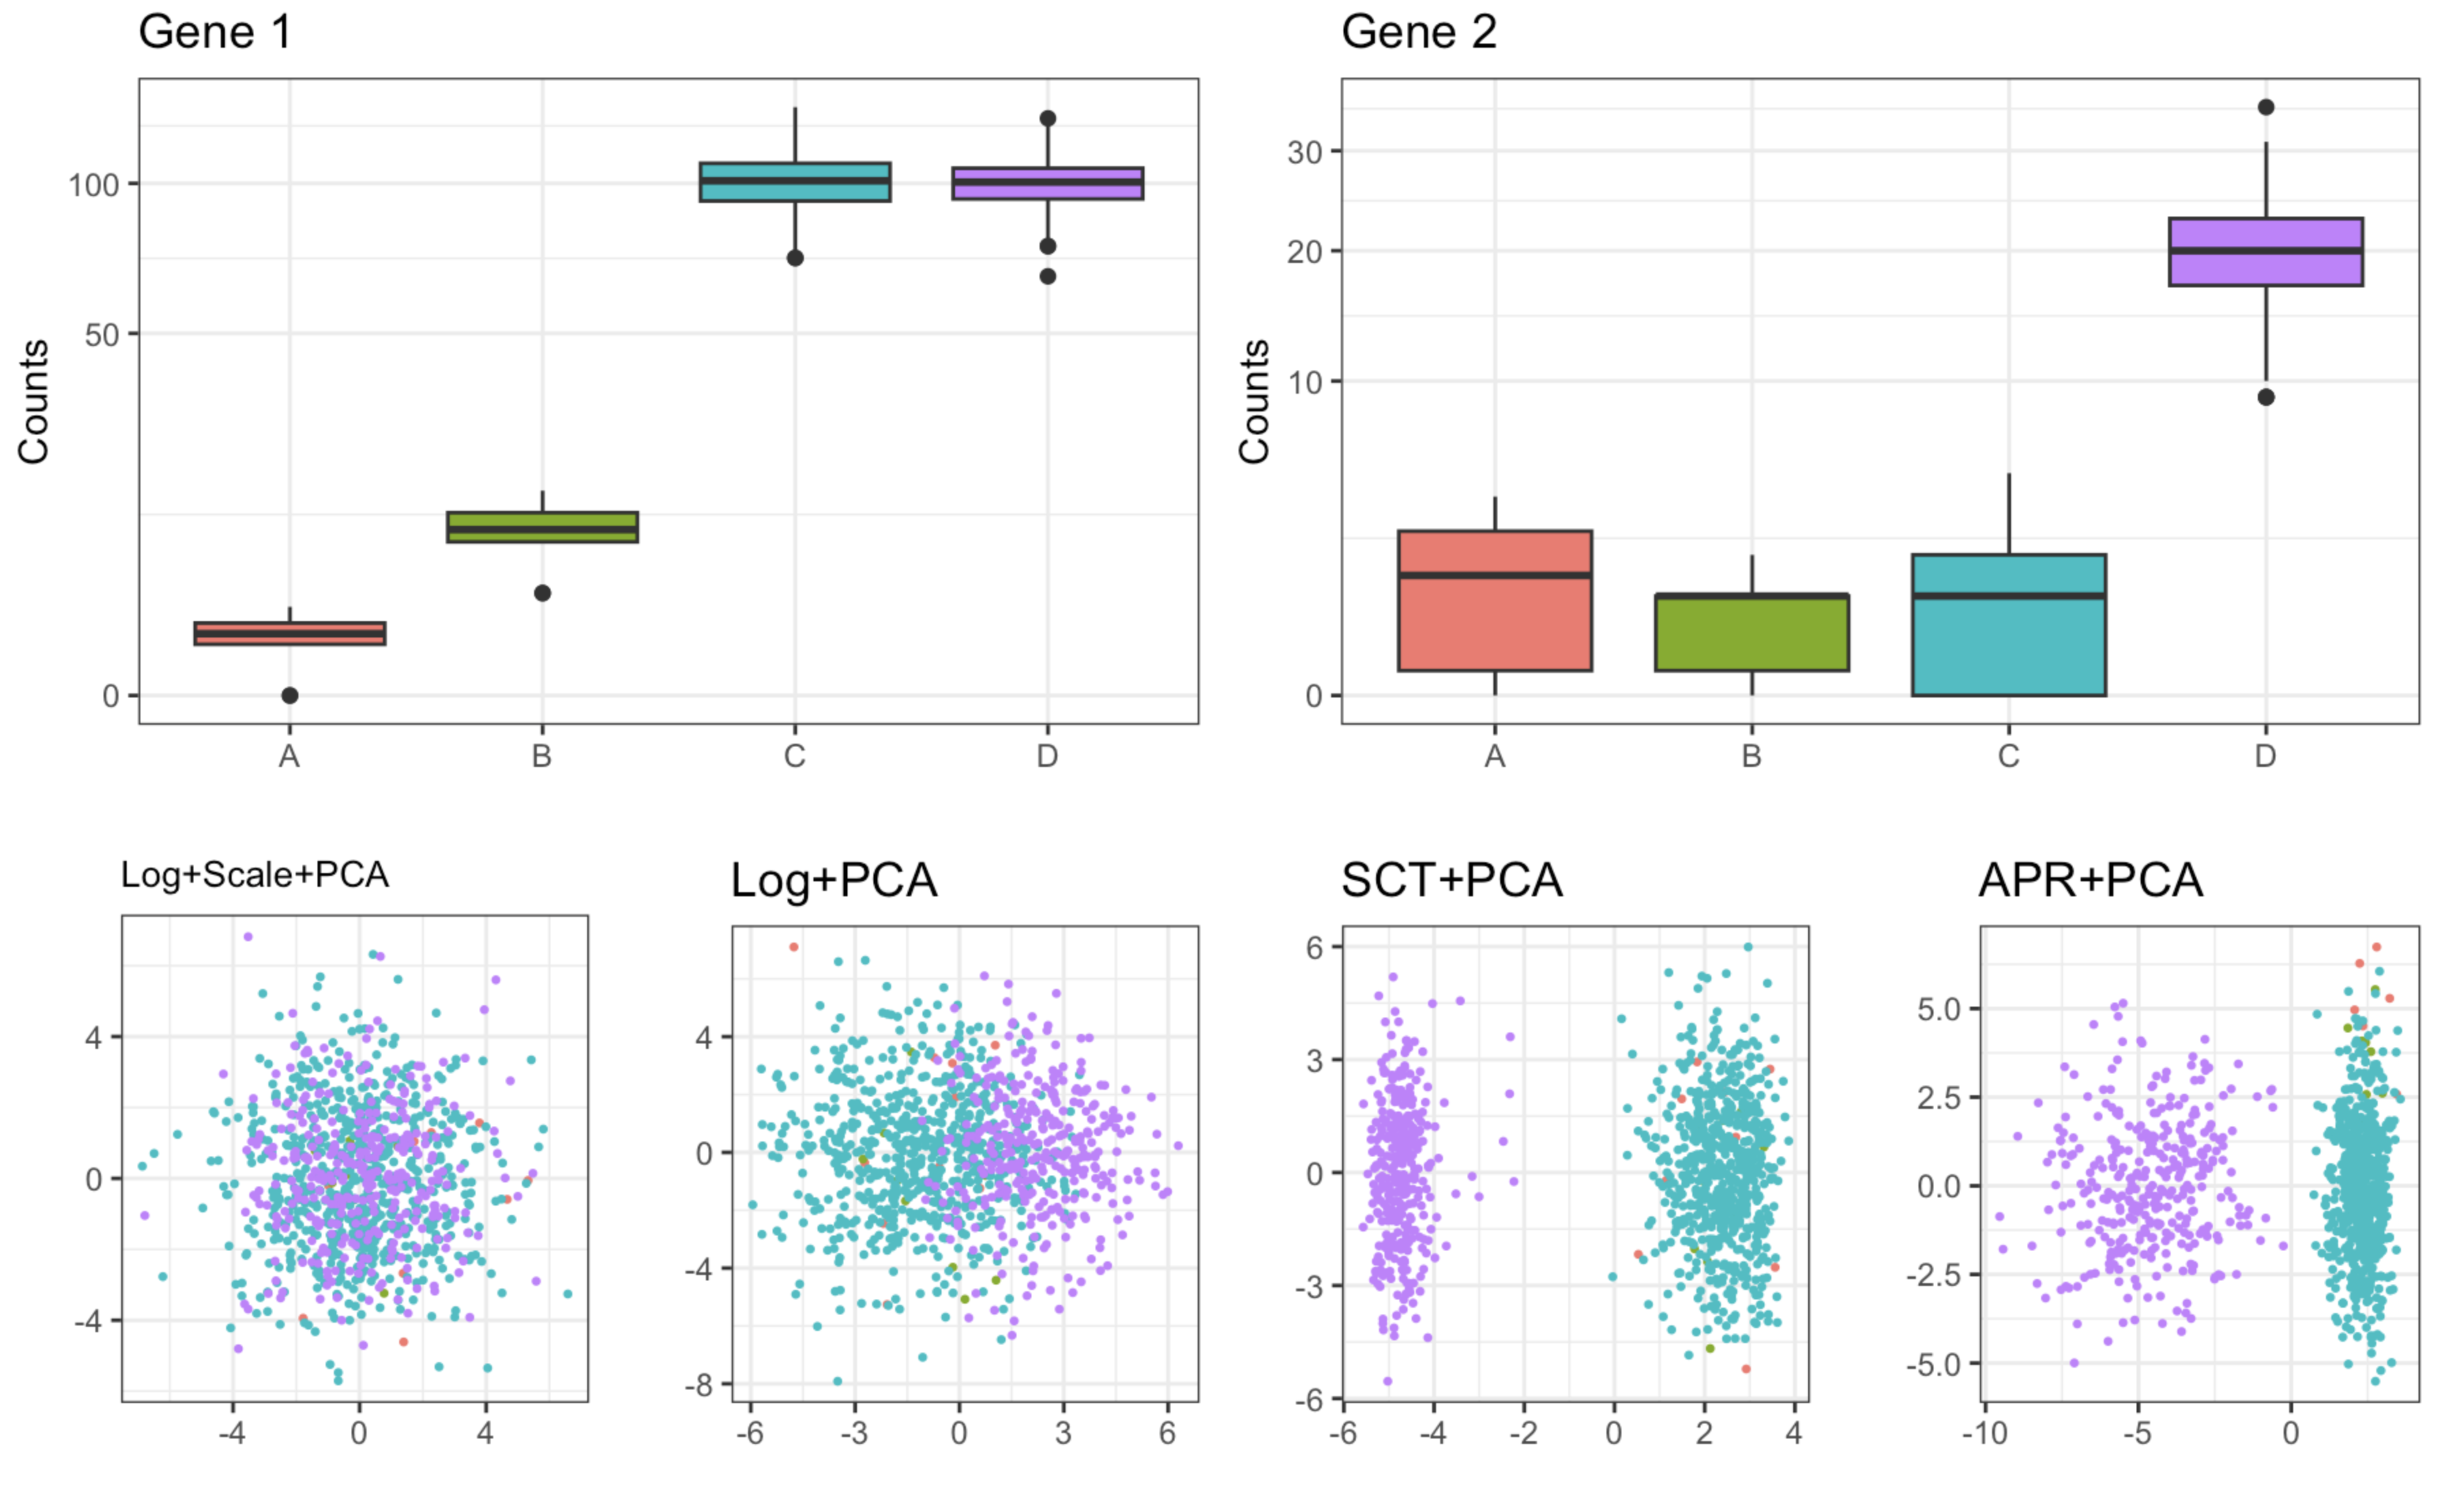
\includegraphics[scale=0.17]{Fig/single_marker_pca.png}
\end{frame}

\begin{frame}{PCA on Pearson residuals is sensitive to changes in baseline expression}

Starting with a dataset of technical replicates, scale each gene (row) by $\kappa_i \sim \text{Expo}(100)$:

\centering 
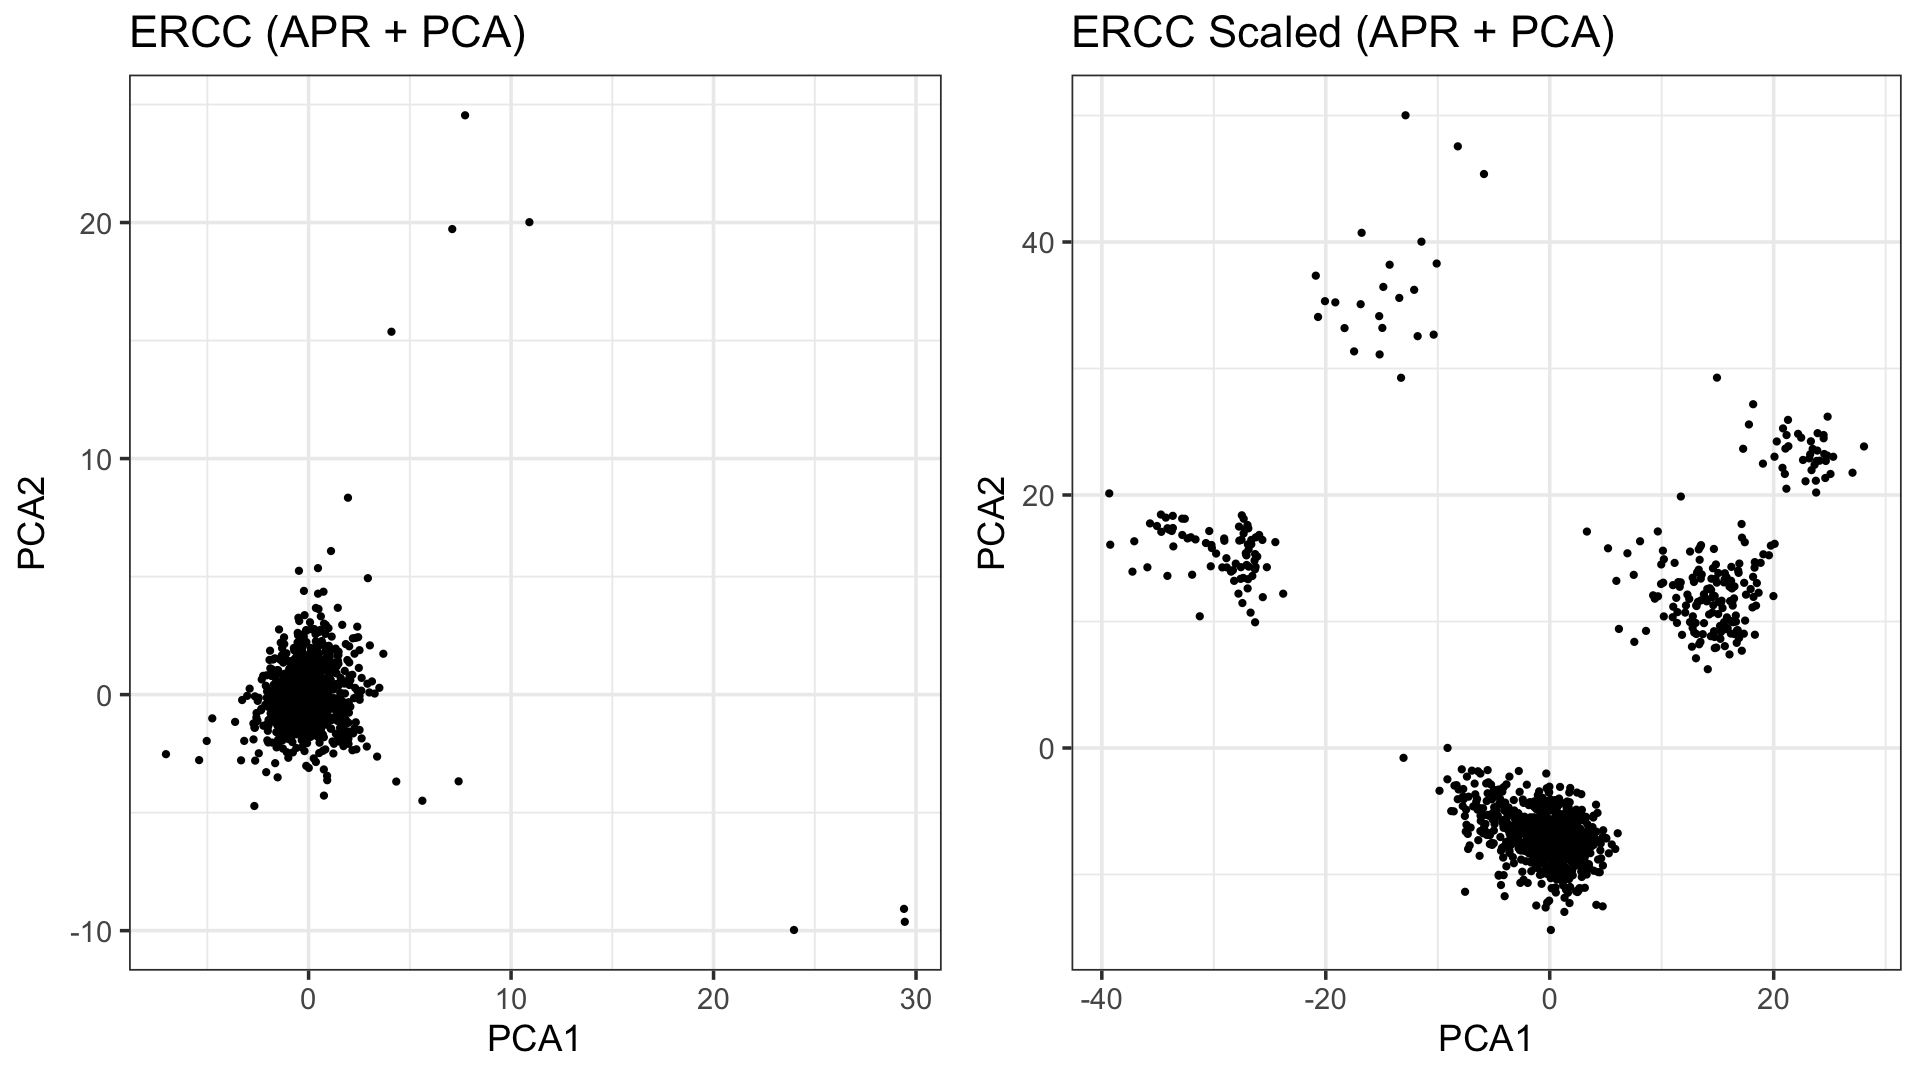
\includegraphics[scale=0.15]{Fig/ercc_scaled_pca.png}

\end{frame}



\begin{frame}{scGBM performs model-based dimension reduction}

\begin{empheq}[box=\fbox]{align*}
Y_{ij} &\sim \text{Pois}(\mu_{ij}) \\
\log(\mu_{ij}) &= \alpha_i + \beta_j + \sum_{m=1}^M \sigma_m u_{im} v_{jm} \\
\sigma_m &\sim \text{Expo}(a)
\end{empheq}

\centering
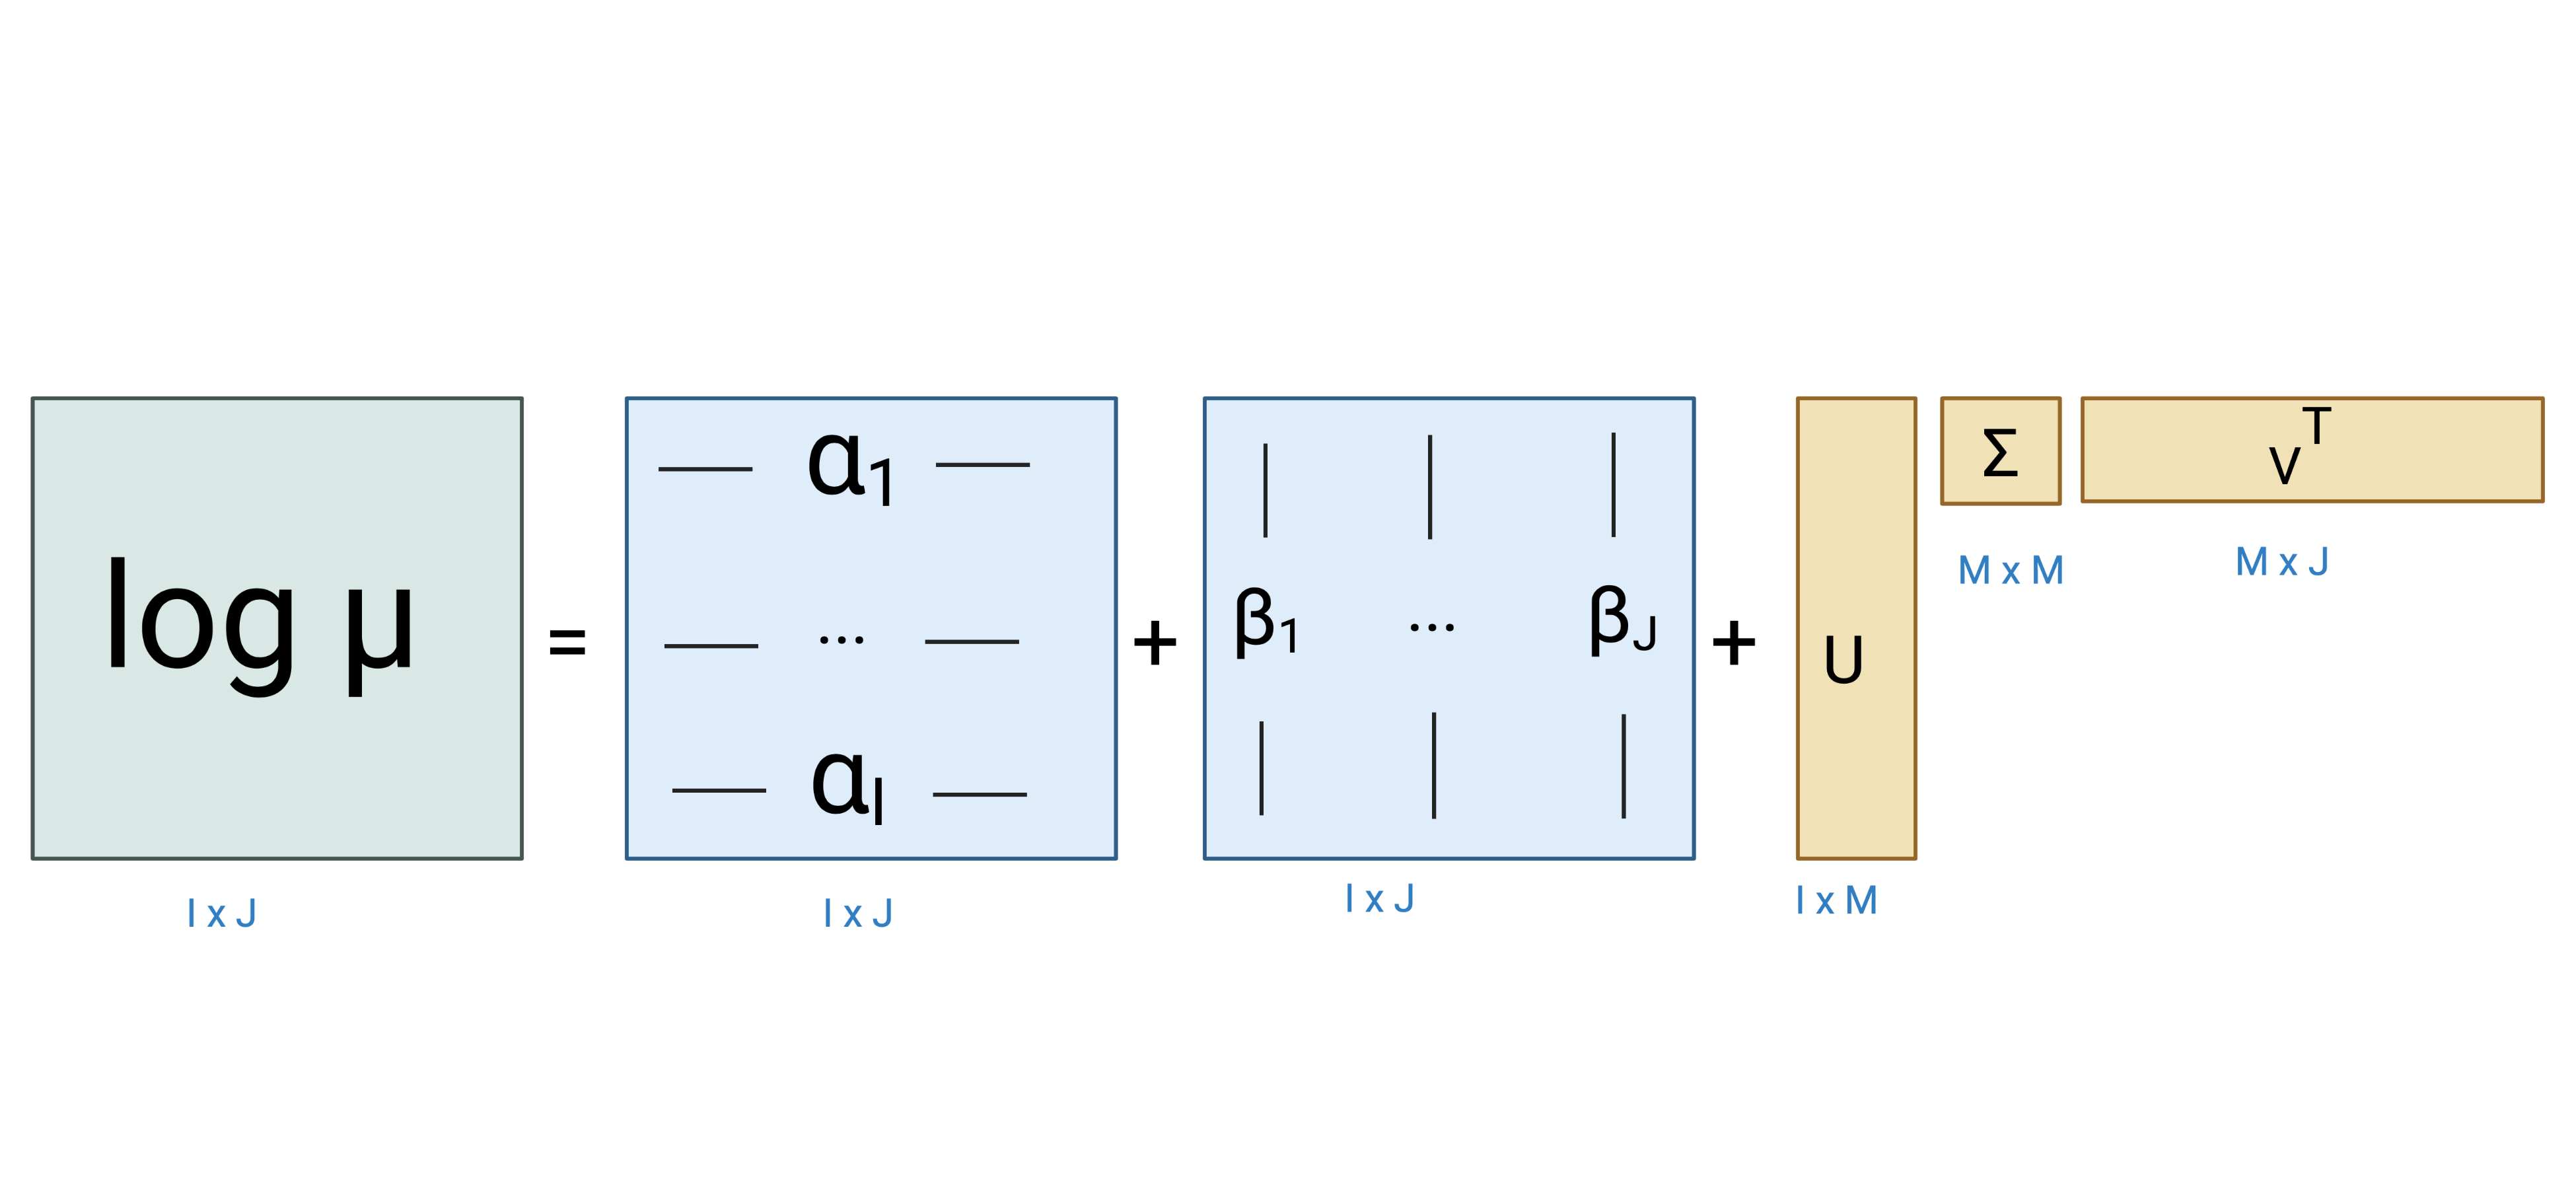
\includegraphics[scale=0.3]{Fig/gbm_model.png}
\raggedright

\vspace{-1em} 

$V \in \R^{J \times M}$ are the low-dimensional cell-embeddings
\end{frame}

\begin{frame}{Estimation with iteratively reweighted singular value decomposition}
Define $\hat{X}^{(t)}$ to be the current estimate of $\hat{U} \hat{\Sigma} \hat{V}^{\top}$. The following update is used for the latent factors:

\begin{equation}
\hat{X}^{(t+1)} = \text{SVD}_{M, 1/a} \left( \hat{X}^{(t)} + \gamma( Y - \hat{\mu})     \right) 
\end{equation}
$\text{SVD}_{M, 1/a}(\cdot)$ computes the rank $M$ truncated SVD and then soft-thresholds the remaining singular values by $1/a$. 

\end{frame}

\begin{frame}{Faster estimation using scGBM-proj}
When $J$ is very large, first estimate $\hat{\alpha}, \hat{U}$ using a smaller subset of cells.

\vspace{3em}

Then holding $\hat{\alpha}$ and $\hat{U}$ fixed, the parameters $\beta$ and $V \Sigma$ can be estimated by fitting $J$ GLMs in parallel. 

\vspace{3em}

By analogy to PCA, we call this the \textit{projection method} (scGBM-proj)

\end{frame}

\begin{frame}{scGBM is faster and more accurate than GLM-PCA}

\end{frame}

\begin{frame}{Rare cell type simulation}
\centering
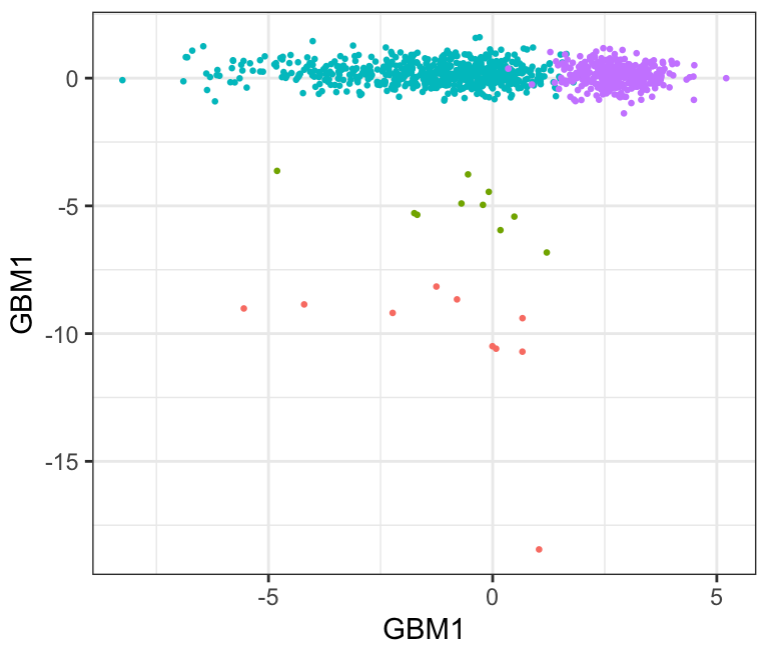
\includegraphics[scale=0.25]{Fig/single_marker_scGBM.png}
\end{frame}

\begin{frame}{ERCC Scaling}

\end{frame}

\begin{frame}{scGBM quantifies uncertainty in the low-dimensional embedding of cells}

\end{frame}

\begin{frame}{Cluster confidence index}

\end{frame}

\begin{frame}{Extending to spatial transcriptomics}

\end{frame}

\begin{frame}{Edge-aware spatial smoothing}

\end{frame}

\begin{frame}{Acknowledgements}
\begin{itemize}
\item Jeff Miller (Harvard Biostatistics)
\item Rafa Irizarry (DFCI Data Science)
\item NIH Cancer Training Grant (REF) 
\end{itemize}
\end{frame}

\begin{frame}{References}
\bibliography{sources}
\end{frame}

\end{document}